\documentclass[twoside, 11pt, a4paper]{article}
\usepackage[latin1]{inputenc}
\usepackage[english]{babel}
\usepackage{amsmath,amsfonts,amssymb,graphicx,parskip}
\usepackage[T1]{fontenc}
%\usepackage{fourierx} % eller lmodern
\usepackage{subfigure}
\usepackage{multirow}
\usepackage{float}
\usepackage{array}
\restylefloat{figure}
\usepackage{algorithm}
\usepackage{algorithmic}
\usepackage{listings}

% for debug utskrift
\newcommand{\debug}[1]{\texttt{#1}}
% for ingen utskrift av kommentarer/debug
%\newcommand{\debug}[1]{}

\DeclareMathOperator{\erf}{erf}
\DeclareMathOperator{\erfc}{erfc}
\DeclareMathOperator{\eps}{\epsilon}
\newcommand{\dee}{\mathrm{d}}

\begin{document}
\LARGE
\begin{center}
TMA4280: Introduction to Supercomputing
\end{center}
\vspace{1in}

\begin{center}
{\bf Parallel I/O using \texttt{MPI-IO}}
\end{center}

\Large
\vspace{0.5in}
\begin{center}
Spring 2014
\end{center}

\vspace{0.5in}

\begin{center}
\copyright Einar M. R{\o}nquist \\
Department of Mathematical Sciences\\
NTNU, N-7491 Trondheim, Norway\\
All rights reserved
\end{center}

\large

\newpage

\section{Introduction}
As HPC applications grow larger and larger as more and more computing resources are
made available, so does the volume of data which needs to be handled, both
on the input and the output side of the application. The process of reading data into
a process or storing data from a process we hereby refer to as \emph{I/O}. The input side is mostly 
a solved problem, in the sense that most operating systems/filesystems added support
for multiple processes reading from the same file years ago.
\begin{figure}[ht]
	\begin{center}
		\includegraphics[width=12cm]{Hard_drive-en}
	\end{center}
	\caption{Illustration of the interior of a hard disk drive. The data is stored on 
			 platters. The data is stored magnetically on these platters by
			 a magnetic device referred to as the \emph{head}. The same device
			 is responsible for retrieving the data when a read operation is issued.
			 Since we only have a single head, HDDs are serial by construction.
			 Image taken from \emph{http://en.wikipedia.org/wiki/Harddrive}.}
	\label{fig:hdd}
\end{figure}
Getting high performance, however, is more involved. For the last thirty years or so,
secondary storage has usually been hard disk drives (commonly abbrevated as \emph{HDDs});
see Figure \ref{fig:hdd} for an illustration of the interior. 
These are mechanical in nature, data is read/written from/to spinning platters through 
a magnetic device referred to as the \emph{head}. Since a HDD only has a single head, it
can only perform a single read/write operation concurrently. 
This means that even though multiple processes can initiate reads concurrently,
they will be performed in serial. Schematically this can be illustrated as in Figure \ref{fig:manyone}.
A HDD only perform at peak levels if data is read or written in large sequential chunks,
since searching for data incur large penalties, as the head has to be repositioned.
In a lot of HPC applications, the access pattern for a single process can seem to
be fairly random from the operating system's point of view, which lead to the I/O being
performed in an inefficient manner. This is due to the fact that the data a particular
process needs is scattered in the file, leading to excessive seeks.
Only when all the I/O performed by the separate processes are considered as a whole,
a sequential pattern can be found. The application developer is often aware of this fact,
and this raises the need for an interface where this information can be given to the 
system. Additional performance can be achieved if a file is stored across multiple 
storage devices. This allows us to harness the aggregated bandwith of the devices;
see Figure \ref{fig:manymany} for an illustration.

\begin{figure}[ht]
	\begin{center}
		\includegraphics[width=12cm]{many-onedisk}
	\end{center}
	\caption{Illustration of I/O where several processes read from a single file.
			 Since a HDD is serial in nature, only one operation can be performed
			 concurrently.}
	\label{fig:manyone}
\end{figure}
\begin{figure}[ht]
	\begin{center}
		\includegraphics[width=12cm]{many-manydisk}
	\end{center}
	\caption{Illustration of I/O where we harness the aggregated bandwith of
			 several devices. Here each process reads its data from a separate
			 physical device, thus the I/O can be performed in parallel.}
	\label{fig:manymany}
\end{figure}

On the output side, things turn more interesting. For years HPC applications solved 
their needs using one of two approaches. The first approach is often referred to as
\emph{post-mortem assembly}; each process dumps its data to a separate file, and 
then custom-tailored code is used to read the data into the next application in the
computational chain, such as visualization software. If implementing the support directly
into the visualization software is not feasible, a separate postprocessing 
application must be written. The second approach, which is also often used, is to 
serialize the I/O. Here one process is given the responsibility of writing the data 
to disc. The other processes then simply send their data to the responsible process, 
in a sequential manner; see Figure \ref{fig:serial}.

\begin{figure}[ht]
	\begin{center}
		\includegraphics[width=12cm]{serial}
	\end{center}
	\caption{Illustration of serialization of the I/O. All processes send their
			 data to process 0, which is responsible for writing the data to secondary
			 storage. Since a harddrive is serial in nature, the total time spent
			 on the operation equals the sum of the time to write the individual data
			 chunks.}
	\label{fig:serial}
\end{figure}

What is common to both of these approaches, is that they necessitate performing (most
of) the I/O in a serial manner. As the data volume grows, this occupies an increasing amount
of the total computational time. Eventually this may become a large bottleneck for the 
parallel performance of your program. The first approach also necessitates performing
substantially more I/O than strictly required, in particular all data is written twice;
first to the separate files and then in a stitched-together fashion as performed by the 
postprocessing application. If the volume of data is substantial, this introduces another
severe bottleneck in your computational chain. The code involved in both of these
approaches is often intricate and prone to errors.
\newpage
It is thus of great interest to be able to store all data in a single file, or at most a 
few files, while avoiding serialization of the I/O both on the application level,
as well as on the physical level, by splitting the file across multiple storage devices. 
Fortunately there are established libraries to enable this. We here consider one
particular example of such an interface, namely the \texttt{MPI-IO} interface. 
As the name implies, this was made part of the official \texttt{MPI} standard back 
in 1998 with the introduction of the \texttt{MPI} 2.0 specification. However, while 
the library strive to yield highly portable code, tuning to the underlying filesystem
(how the data is stored on the hard disk drive(s)) is unavoidable when it comes to 
obtaining high performance. One example of such a file system is the \emph{general parallel 
filesystem}, \texttt{GPFS} for short, developed by IBM 
during the last 10 years. This is in use on \texttt{NOTUR} systems (\emph{Kongull}, \emph{vilje}). Since such tuning is somewhat 
technical and beyond the intention of this document, this will not be discussed in 
detail in the following.

\section{\texttt{MPI-IO} - basic concepts}
\texttt{MPI-IO} is the part of the official \texttt{MPI} standard which covers parallel I/O.
It offers a simple, natural interface for expressing parallelism in I/O. Informing
the system about the underlying distributed nature of an I/O call enables the system
to make good choices about how the I/O is performed on a lower level. 
We first consider the simplest case; I/O that is sequential on each process.

\subsection{Sequential I/O}
We here consider sequential I/O, namely writing a contiguous slice 
of data from a set of separate processes. The data storage pattern in this case is
fairly trivial, as illustrated in Figure \ref{fig:contigousstorage}. An example
where such a pattern could occur, is if we have partitioned a matrix in a strip
fashion across the processes; see Figure \ref{fig:strip} for an illustration.

\begin{figure}[ht]
	\begin{center}
		\includegraphics[width=12cm]{slicedvector}
	\end{center}
	\caption{Illustration of an I/O operation where a contiguous piece of data
			 is sliced into chunks. A single contiguous chunk of data is then
			 written by each process. All the chunks are written to the same file.}
	\label{fig:contigousstorage}
\end{figure}

If you are familiar with standard \texttt{POSIX} I/O calls, the basic form
of the \texttt{MPI-IO} code should look very familiar.
On each process we start by opening a handle to the file we want to write to, in
this case called ``datafile''.
\lstinputlisting[language=C]{open-handle.c}
A file handle is described by a variable of type \emph{MPI\_File}. In addition to
which file we want to open, we also have to specify flags which the system use to both 
control which accesses are allowed, as well as for directives which help increase performance.
Here we only specify flags of the former class, in particular, we only want 
to write to the file (by specifying the flag \emph{MPI\_MODE\_WRONLY}) and 
we want the file to be created if it doesn't already exist (by specifying the flag 
\emph{MPI\_MODE\_CREATE}). The function includes an
additional parameter of type \emph{MPI\_Info}. For now we pass the builtin value
\emph{MPI\_INFO\_NULL} which can be used when we do not want to pass any data in
this field. We will briefly comment on this later.

With the file opened, we proceed with writing the data. In this example,
our data is an array of doubles named \emph{vec}. The total global array length
is \emph{N}, which means we have $N/size$ elements per process (here \emph{size}, as
usual, denotes the number of processes, while \emph{rank} denotes the process number).
We first seek to the appropriate offset in the file, then write the chunk of data.
\lstinputlisting[language=C]{separate-handle-write.c}

An alternative way of doing the same operation, is to use the \emph{explicit offset}
\emph{MPI\_File\_Write\_at} function. This is mainly a matter of convenience, i.e.
it allows to do the same operation with less code, in particular, we avoid the 
seek call;
\lstinputlisting[language=C]{explicit-offset-write.c}

Common to both of these alternatives is that they use individual I/O calls on each
process. If the underlying system is smart, it should be able to recognize the access
pattern. If we want to make sure that the system notices this fact, we can use
\emph{collective} calls. In particular, consider
\lstinputlisting[language=C]{collective-write.c}
Here we inform the system that we are performing a collective write among all the
processes. This allows the system to do additional coordination of how the I/O is 
performed. However, it comes at a cost. In particular, all processes will stall 
until the entire I/O operation is completed across all the processes, while
using individual handles allows the program flow to continue on each process as
soon as their share of the I/O has been performed.

Another convenience function in the context of collective calls is \emph{shared} writes.
In addition to containing info about the position on the individual processes, a 
\emph{MPI\_File} variable also contains info about a shared state between all the
processes. Here, with our simple data layout, this can be exploited to make the code
particularly simple. We simply have to do
\lstinputlisting[language=C]{shared-write.c}
This function use the shared state in the filepointer. Upon the call, the writes are
performed in order according to process rank.

Finally we have to close our file. This is performed by doing
\lstinputlisting[language=C]{close.c}

\section{Non-sequential I/O - fileviews}
In the previous section we considered an extremely simple data access pattern. Such a
pattern is only the predominant one in simple codes. Usually the access patterns
in real applications are much more involved. Programming such access patterns naively 
using many seeks and many small writes is certainly a possibility, however hardly something 
we would recommend. In addition to being highly error prone, it would also make it 
very hard for the system to get a proper view of the collective I/O performed across 
the processes.

For purposes of easy presentation, we here again consider a simple data layout.
In particular, consider a vector split in a cyclic manner, see Figure
\ref{fig:cyclicvector}. 

\begin{figure}[ht]
	\begin{center}
		\includegraphics[width=12cm]{splitvector}
	\end{center}
	\caption{Illustration of cyclic partition of a vector. Each process
			 write a single number, followed by a gap of $size-1$ numbers.
			 This pattern repeats for the extent of the data.}
	\label{fig:cyclicvector}
\end{figure}
If we perform this I/O naively, each process would write a single number, perform
a seek, write another number and so on. Such small writes followed by seeks makes
it very hard for the system to optimize the I/O. \texttt{MPI-IO} offers a much better
approach. It builds on the \texttt{MPI} machinery for constructing custom types.
While these datatypes are used to describe the data layout in memory in standard 
\texttt{MPI} functions, they are here used to describe the data layout on secondary
storage. From each process, the data access pattern is one number followed
by a gap of \emph{size-1} numbers. We can describe such a pattern in a \texttt{MPI}
datatype as
\lstinputlisting[language=C]{createsplitview.c}
We here use the function
\[
	MPI\_Type\_create\_resized(origtype,lb,extent,newtype)
\]
to create the gap. We set \emph{lb} (lower bound) = 0 to indicate that we want the real
data to start at the beginning of the new data type. We then extend this to be
size doubles long. We can now attach this view of the data to the file using
the function
\newpage
\[
	MPI\_File\_set\_view(fh,disp,datatype,viewtype,encoding,info)
\]
as
\lstinputlisting[language=C]{setsplitview.c}
Note the usage of the \emph{disp} field. This field describes an offset that the
process sees as the start of the file. By setting this offset equal to position
of the first number the particular process should write to the file, the
data access pattern (\emph{MPI\_Datatype}) we described further up is exactly
the same on each process. With this configured, writing the data to the file in 
the proper pattern is now just a normal write call, e.g. using separate handles
\lstinputlisting[language=C]{writesplitview.c}
A code demonstrating this can be found in Appendix \ref{app:cyclicvector}.

We stress that there is nothing stopping you from using different fileviews on
the different processes. In fact, we now move on to consider a particular case where
this is needed, namely when we want to handle arrays/matrices partitioned over
several processes.

\begin{figure}[ht]
	\begin{center}
		\subfigure{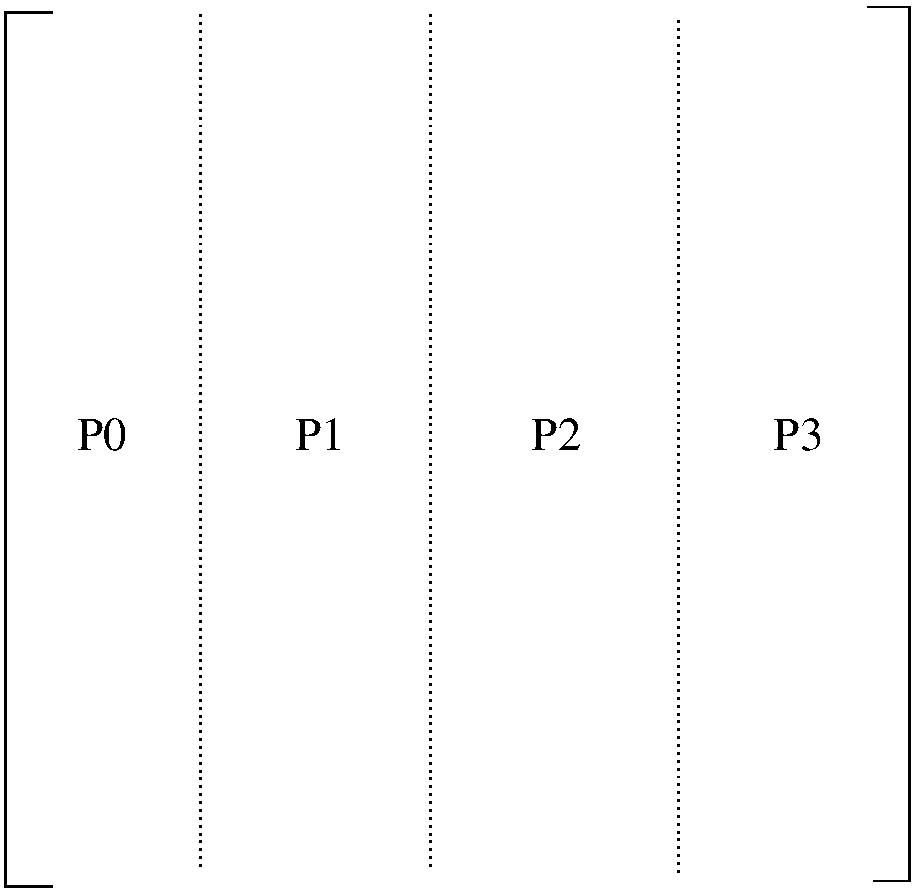
\includegraphics[width=6cm]{strip}\label{fig:strip}}
		\subfigure{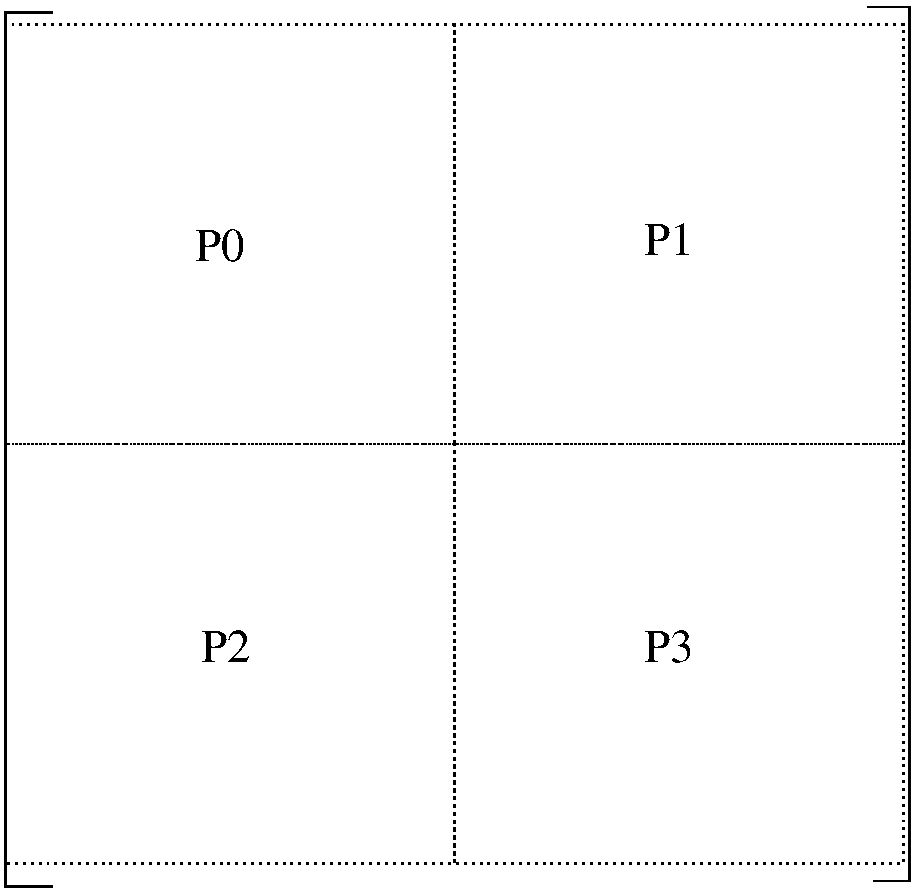
\includegraphics[width=6cm]{block}\label{fig:block}}
	\end{center}
	\caption{Illustration of two possible ways a 2D array can be distributed
			 across several processes. In (a) each process is responsible for
			 a number of whole columns. In (b) each process is instead reponsible
			 for a sub-block of the array.}
	\label{fig:darrays}
\end{figure}

\section{Non-sequential I/O - distributed arrays}
In HPC applications, your data usually consists of matrices (2D arrays) or 3D arrays.
This fact has not gone past the \texttt{MPI} creators, and as such \texttt{MPI}
contains machinery for generating partioning of such arrays in a semi-automatic way.
Since \texttt{MPI-IO} is built on \texttt{MPI}, this machinery is also extremely
useful when we want to write the data to secondary storage. We now show how to
employ these utility functions to make writing distributed arrays to disc as simple
as performing a single write call.

\texttt{MPI} names such distributed arrays \emph{darray} for short. The available
functions are heavily inspired by the \texttt{High Performance Fortran} standard,
\texttt{HPF} for short. This is a standard which aims to make developing HPC software 
easier through semi-automatic parallelization. In this context, the most important parts 
of this standard is its conventions for array partitioning 
strategies and process topologies, since \texttt{MPI} follows the same conventions.
The two possible partitionings of most interest in this context is illustrated in 
Figure \ref{fig:darrays}. As we will show shortly, these are to some extent similar.

\begin{figure}[ht]
	\begin{center}
		\includegraphics[width=12cm]{splitdomain}
	\end{center}
	\caption{A block partition of a 2D array with the pieces of information
			we need to classify this partitioning.}
	\label{fig:splitdomain}
\end{figure}
\newpage
We now show how to use the \texttt{MPI} machinery to easily partition an array.
Consider Figure \ref{fig:splitdomain}. We here have a 2D array we want to partition
across 6 \texttt{MPI} processes. The figure contains the pieces of information
we need to classify a partitioning;
\begin{itemize}
	\item A global topology - here a Cartesian topology expressed as the number 
		  of processes along each dimension (here 2 and 3, respectively).
	\item Location of a particular domain in the topology, again
		  this can be expressed as an integer along each dimension.
	\item A mapping of the available processes onto the topology.
\end{itemize}

The first useful function is \emph{MPI\_Dims\_create}. This function generates a 
Cartesian partioning of your processes according to a the rules set by \texttt{HPF}.
\lstinputlisting[language=C]{dimsblock.c}
The initialization of the entries in sizes prior to calling the function is important.
In particular, the function will only operate along a dimension $i$ where sizes[i] = 0
on function entry. While this interface makes it very easy for the programmer to
make errors (i.e. forgetting to initialize the array properly), it also has advantages.
For instance, if we instead want to divide our matrix in a strip fashion, we can do
\lstinputlisting[language=C]{dimsstrip.c}
Of course, if we only have one partitioned dimension in our array,
generating the topology is trivial. The nice thing with doing it like this is that it
allows us to use fairly similar code, whether we want a strip or a block partitioning of 
the arrays; see Figure \ref{fig:darrays}. We stress that this only generates the
\emph{topology} (or partitioning structure), it does not in any way depend on the array dimensions. 
Upon return from the function the \emph{dims} array contains the number of processes
used in the separate directions, 2 and 3, respectively, in our example.

Now we have a topology describing the layout of our processors, or rather how many
processors the dimensions are split over. Still, each
processor needs to know where they are located in this topology. To be able to decide this,
we first have to create a communicator group which has the (Cartesian) topology attached.
This can be achieved by
\lstinputlisting[language=C]{comm.c}
The \emph{periodic} array is an integer array with either 0 or 1 as entries. These are used to
specify whether or not the domain is periodic in the particular dimension, which 
is not the case with a standard 2D array as the one we consider here.
Upon return from the function, the \emph{comm} variable holds the new communicator info.
This can now be used wherever \texttt{MPI} expects a communicator (i.e. instead of
the builtin \emph{MPI\_COMM\_WORLD} we have used previously).
This takes care of mapping the processes onto the topology.

Finally, each process can then find their location in the topology using
\lstinputlisting[language=C]{coord.c}
Upon return from the function, the \emph{coords} array holds the coordinates. In our example,
it would for instance hold 1 and 2 when called on process 5.

With the problem partitioning taken care of, it is time to tie this into \texttt{MPI-IO}.
\texttt{MPI} includes functions to describe such a distributed array layout in memory,
which usually are useful when you want to collect a whole array on a single process.
Collecting all data on a single process is exactly what we want to perform when
we write this to secondary storage, the only difference is that in our case this
``process'' is the file on secondary storage. Thus we can use the functions originally
intended for describing the data layout in memory to instead generate the fileviews
on the separate processes. The function we need is
\[
	\begin{split}
		MPI\_Type\_create\_darray(size,rank,dims,gsizes, \\
								  distribs,dargs,sizes, \\
								  order,etype,newtype).
	\end{split}
\]
Here \emph{size} is the size of the communicator (typically the number of processes),
\emph{rank} the process rank within the communicator, \emph{dims} the number of
dimensions in the array (2 for a matrix), \emph{gsizes} the sizes of the global array
along the dimensions, \emph{distribs} distribution strategies along the dimensions,
\emph{dargs} a distribution strategy parameter (can usually be set to \emph{MPI\_DISTRIBUTE\_DFLT\_DARG}), 
\emph{dims} the topology results as obtained using \emph{MPI\_Dims\_create},
\emph{order} describes the array layout in memory (\emph{MPI\_ORDER\_C} or
\emph{MPI\_ORDER\_FORTRAN}), \emph{etype}
the datatype of the array entries and finally \emph{newtype} our new datatype.

The most interesting of these are the \emph{distribs} array. This array contains
the chosen distribution strategy along each dimension. The strategy can be one of
\begin{enumerate}
	\renewcommand{\theenumi}{$\bullet$}
	\renewcommand{\labelenumi}{\theenumi}
	\item \bf MPI\_DISTRIBUTE\_NONE: \rm  Here no partitioning of the array is applied along 
	this dimension.
	\item \bf MPI\_DISTRIBUTE\_CYCLIC: \rm Here a cyclic partitioning of the array is applied
	along this dimension.
	This distribution is often used in \texttt{HPF} codes. We do not consider it here.
	\item \bf MPI\_DISTRIBUTE\_BLOCK: \rm Here a block partitioning of the array is applied
	along this dimension.
\end{enumerate}
For instance, if we want to block-partition an array of doubles with size $N\times N$
stored according to \texttt{C} convections (row-major storage), we do
\lstinputlisting[language=C]{createarrayview.c}
If we now set this datatype as the fileview on the individual processes as described
earlier, we can now write them to disc using a single write call. This is much
much easier than the alternative using separate write/seek calls.

A code that handles both strip and block partitioned arrays can be found in
Appendix \ref{app:darray}.
\newpage
\section{Non-blocking I/O - overlapping I/O and computations}
On modern architectures HDDs can write/read data (almost) completely on their own
using a technique known as \emph{Direct Memory Access}, \emph{DMA} for short.
This means that while we are writing/reading data the CPU is mostly an idle
observer. This is not good for program efficiency, ideally we would like
to keep the CPUs saturated with work whenever we can.
\texttt{MPI-IO} also offers facilities to remedy this,
namely \emph{non-blocking} I/O. All classes of I/O calls have non-blocking
equivalents, to simplify the presentation we here only consider using
individual handles on each process.

The basic idea can be summarized in the following piece of (somewhat)
abstract code;
\lstinputlisting[language=C]{overlapping.c}
We have here replaced the \emph{MPI\_File\_write} function with a call
to \emph{MPI\_File\_iwrite}, which is the nonblocking equivalent. This
call initiates the I/O operation, then immediately returns. The function
takes an additional parameter of type \emph{MPI\_Request}. Upon the return
from the function call, this will be updated with information which 
identifies the I/O operation. We are now free to perform additional
calculations, as long as the data we just requested written to secondary 
storage is not touched by this code. In particular, the vector \emph{vec}
cannot be updated in the \emph{doSomething()} call. When we get to a point 
where we need write access to the vector \emph{vec} again, we do a call to 
\emph{MPI\_Wait} with the \emph{MPI\_Request} variable as a parameter.
This function will only return once it is safe to reuse \emph{vec}.
Note that a call to a nonblocking I/O function \emph{ALWAYS} needs
to be accompanied with a call to \emph{MPI\_Wait}, even if you
do not plan to reuse the memory area you requested written to secondary storage.
\newpage
\section{Tuning for performance}
As mentioned in the introduction, a program using \emph{MPI-IO} needs to be tuned
to the particular underlying filesystem if we want the best performance.
This tuning can be divided in two classes.
\noindent
\begin{enumerate}
	\renewcommand{\theenumi}{$\bullet$}
	\renewcommand{\labelenumi}{\theenumi}
	\item \bf Directives \rm - This class of tuning parameters are something an
			  implementation has to obey. One example of such a tuning parameter is
			  the flag \emph{MPI\_MODE\_SEQUENTIAL} which can be passed upon
			  opening the file, just like we passed e.g. \\
			  \emph{MPI\_MODE\_WRONLY} earlier. This tells the system
			  that only sequential access to the data is performed, information
			  which can be used to optimze the I/O.
	\item \bf Hints \rm - These are, as the name indicates, just hints to the
			  implementation. If an implementation does not support/utilize
			  a particular hint, they can just be silently ignored. This
			  is the framework in which vendor specific/filesystem specific tuning
			  can be performed.
\end{enumerate}

These hints are passed to the implementation in a variable of type \emph{MPI\_Info}.
First we need to create the appropriate structure, this is achieved through
\lstinputlisting[language=C]{infoinit.c}
We can now set hints in this structure. A hint is a pair of (key,value) strings.
We add such a hint to our \emph{MPI\_Info} variable using the function
\[
	MPI\_Info\_set(info,key,value)
\]
Such a call might look like
\lstinputlisting[language=C]{infoset.c}

Once we have added all hints we want to the \emph{MPI\_Info} variable, we can now
pass these hints to the implementation upon opening a file.
\lstinputlisting[language=C]{infoopen.c}
We here pass our \emph{MPI\_Info} variable instead of \emph{MPI\_INFO\_NULL} as earlier.

\section{Further reading}
You can find the \texttt{MPI-IO} standard as well as tutorials on the official
\texttt{MPI} homepage \emph{http://www.mpi-forum.org/}. Some useful papers and slides
can be found at \\
\emph{https://computing.llnl.gov/?set=code\&page=sio\_papers\_presentations}.
These are, in particular, of interest if you want extensive knowledge about using
\texttt{MPI-IO} on top of \texttt{GPFS}.

\bf Acknowledgement\rm. J{\o}rn Amundsen gave some useful pointers while this
document was written, in particular the link to llnl.gov. Tobias Arrskog 
helped with proof reading. The document is written by Arne Morten Kvarving.
Your assistance was greatly appreciated. 

\nocite{towards}
\nocite{mpi-io}
\nocite{mpi-io2}
\bibliography{referanser}
\bibliographystyle{plain}
\newpage
\appendix
\section{Storage of a cyclic-partitioned vector using \texttt{MPI-IO}.}
\label{app:cyclicvector}
\lstinputlisting[language=C]{fileview.c}
\newpage
\section{Storage of a block/strip partitioned array using \texttt{MPI-IO}.}
\label{app:darray}
\lstinputlisting[language=C]{combined.c}

\end{document}
